\documentclass{standalone}
\usepackage{tikz}
\usetikzlibrary{patterns, positioning}
\usepackage[sfdefault]{ClearSans} %% option 'sfdefault' activates Clear Sans as the default text font
\usepackage[T1]{fontenc}

\begin{document}
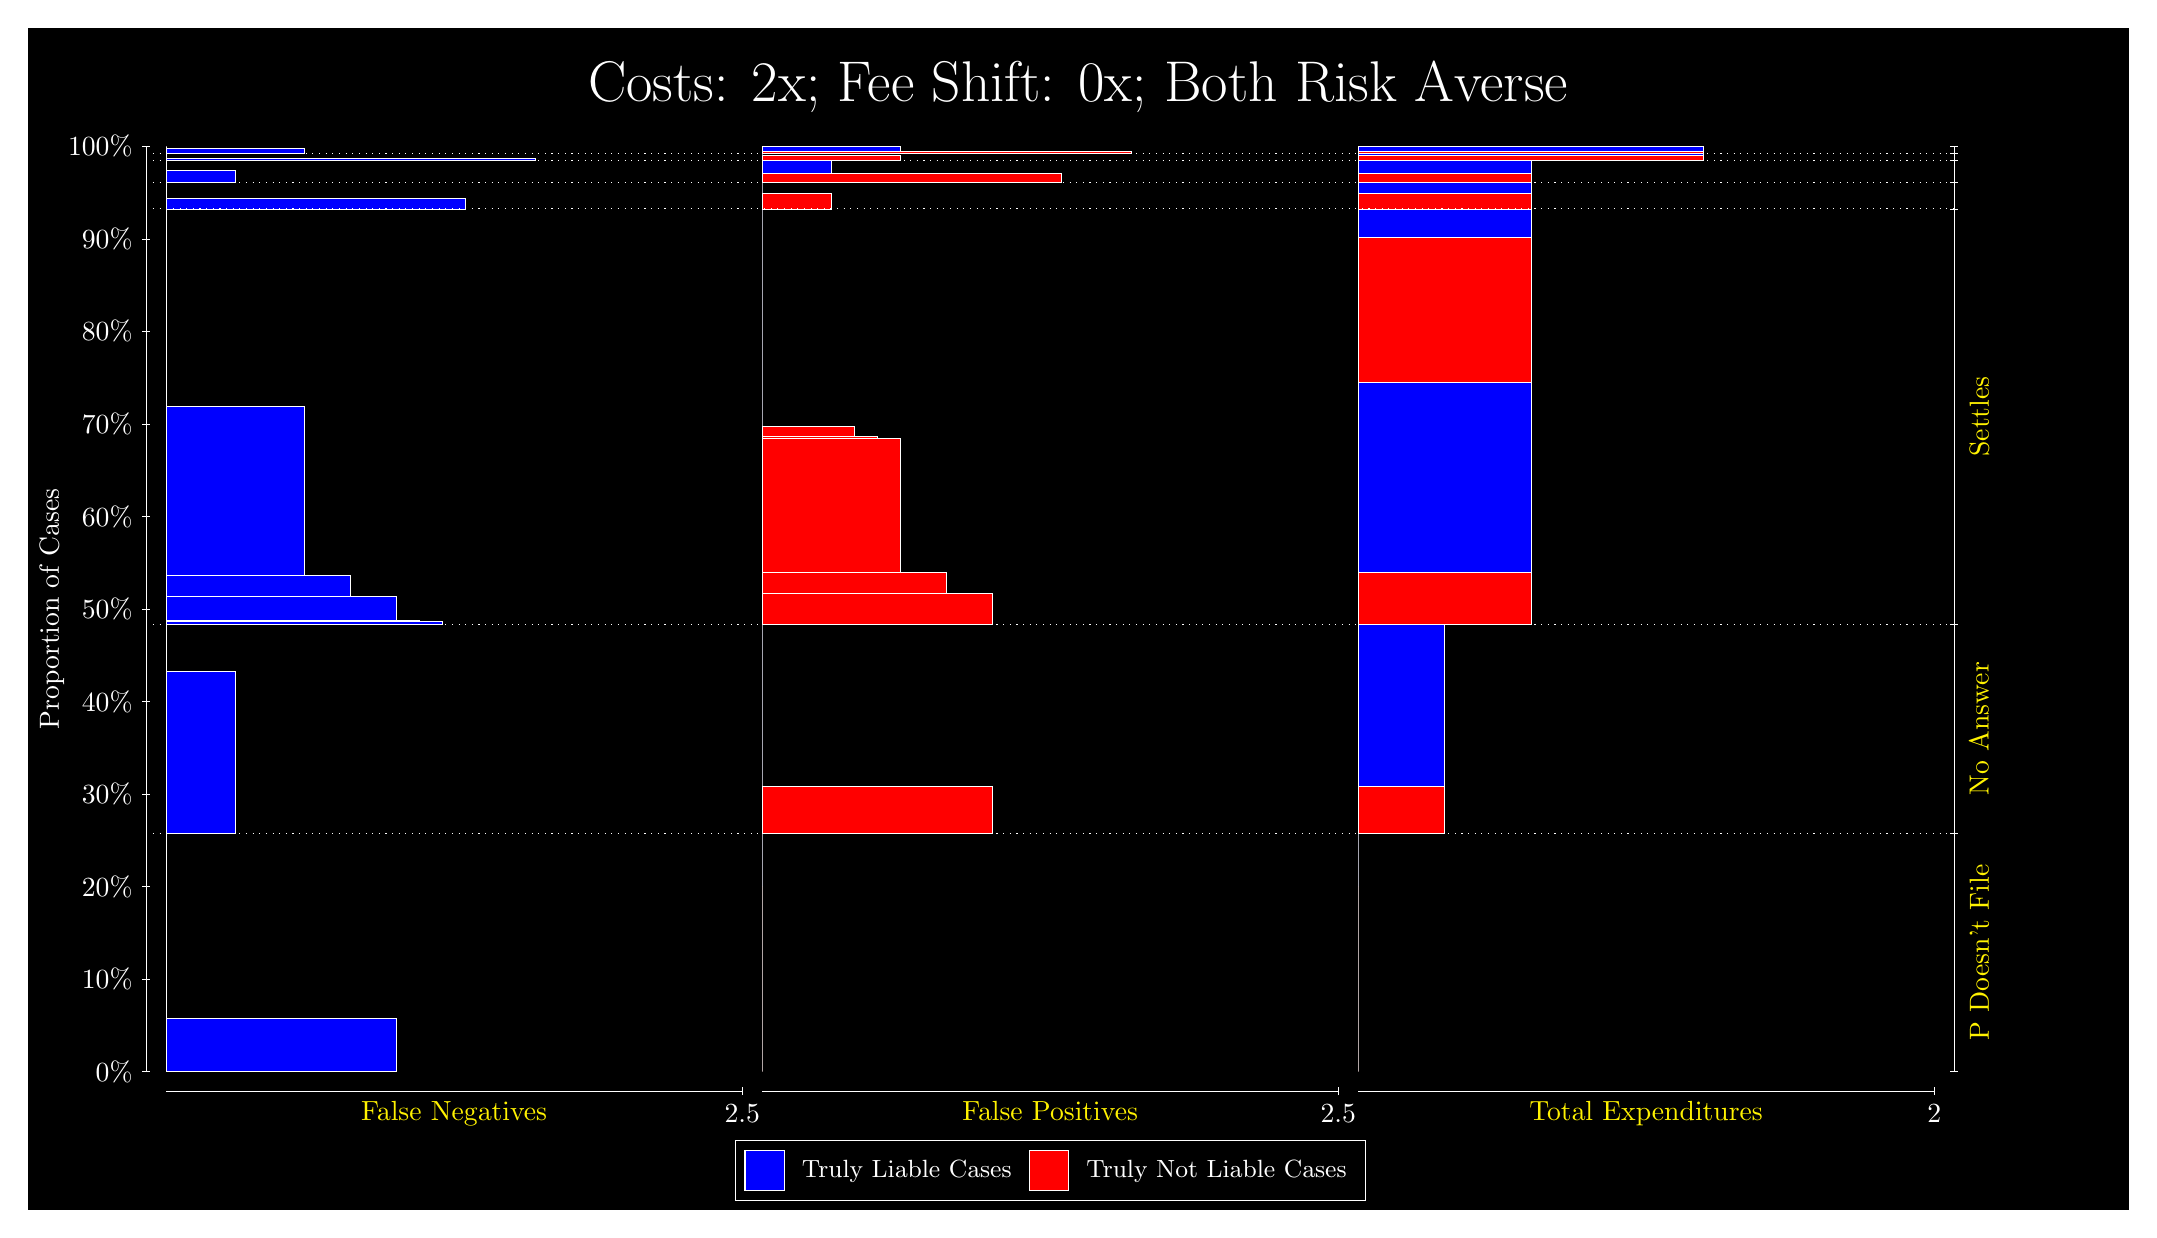
\begin{tikzpicture}
\draw[fill=black] (0,0) rectangle (26.667,15);
\draw[text=white] (0,13.5) rectangle (26.667,15) node[midway] {\huge Costs: 2x; Fee Shift: 0x; Both Risk Averse};
\draw[white, very thin] (1.5,1.75) -- (1.5,13.5);
\node[rotate=90, text=white, anchor=center] at (0.3, 7.625) {Proportion of Cases};
\draw[white, very thin] (1.45,1.75) -- (1.55,1.75);
\node[text=white, anchor=east] at (1.45, 1.75) {0\%};
\draw[white, very thin] (1.45,2.925) -- (1.55,2.925);
\node[text=white, anchor=east] at (1.45, 2.925) {10\%};
\draw[white, very thin] (1.45,4.1) -- (1.55,4.1);
\node[text=white, anchor=east] at (1.45, 4.1) {20\%};
\draw[white, very thin] (1.45,5.275) -- (1.55,5.275);
\node[text=white, anchor=east] at (1.45, 5.275) {30\%};
\draw[white, very thin] (1.45,6.45) -- (1.55,6.45);
\node[text=white, anchor=east] at (1.45, 6.45) {40\%};
\draw[white, very thin] (1.45,7.625) -- (1.55,7.625);
\node[text=white, anchor=east] at (1.45, 7.625) {50\%};
\draw[white, very thin] (1.45,8.8) -- (1.55,8.8);
\node[text=white, anchor=east] at (1.45, 8.8) {60\%};
\draw[white, very thin] (1.45,9.975) -- (1.55,9.975);
\node[text=white, anchor=east] at (1.45, 9.975) {70\%};
\draw[white, very thin] (1.45,11.15) -- (1.55,11.15);
\node[text=white, anchor=east] at (1.45, 11.15) {80\%};
\draw[white, very thin] (1.45,12.325) -- (1.55,12.325);
\node[text=white, anchor=east] at (1.45, 12.325) {90\%};
\draw[white, very thin] (1.45,13.5) -- (1.55,13.5);
\node[text=white, anchor=east] at (1.45, 13.5) {100\%};

\draw[white, very thin] (24.457,1.75) -- (24.457,13.5);
\draw[white, very thin] (24.407,1.75) -- (24.507,1.75);
\node[anchor=west] at (24.407, 1.75) {};
\draw[white, very thin] (24.407,4.7779) -- (24.507,4.7779);
\node[anchor=west] at (24.407, 4.7779) {};
\draw[white, very thin] (24.407,7.4319) -- (24.507,7.4319);
\node[anchor=west] at (24.407, 7.4319) {};
\draw[white, very thin] (24.407,12.705) -- (24.507,12.705);
\node[anchor=west] at (24.407, 12.705) {};
\draw[white, very thin] (24.407,13.039) -- (24.507,13.039);
\node[anchor=west] at (24.407, 13.039) {};
\draw[white, very thin] (24.407,13.321) -- (24.507,13.321);
\node[anchor=west] at (24.407, 13.321) {};
\draw[white, very thin] (24.407,13.41) -- (24.507,13.41);
\node[anchor=west] at (24.407, 13.41) {};
\draw[white, very thin] (24.407,13.5) -- (24.507,13.5);
\node[anchor=west] at (24.407, 13.5) {};

\draw[white, very thin, fill=blue] (1.75,1.75) rectangle (4.6775,2.4245);
\draw[white, very thin, fill=red] (1.75,2.4245) rectangle (1.75,4.7779);
\draw[white, very thin, fill=blue] (1.75,4.7779) rectangle (2.6283,6.8321);
\draw[white, very thin, fill=red] (1.75,6.8321) rectangle (1.75,7.4319);
\draw[white, very thin, fill=blue] (1.75,7.4319) rectangle (5.2631,7.4727);
\draw[white, very thin, fill=blue] (1.75,7.4727) rectangle (4.9703,7.4788);
\draw[white, very thin, fill=blue] (1.75,7.4788) rectangle (4.6775,7.7874);
\draw[white, very thin, fill=blue] (1.75,7.7874) rectangle (4.092,8.0579);
\draw[white, very thin, fill=blue] (1.75,8.0579) rectangle (3.5065,10.194);
\draw[white, very thin, fill=red] (1.75,10.194) rectangle (1.75,12.705);
\draw[white, very thin, fill=blue] (1.75,12.705) rectangle (5.5558,12.838);
\draw[white, very thin, fill=red] (1.75,12.838) rectangle (1.75,13.039);
\draw[white, very thin, fill=blue] (1.75,13.039) rectangle (2.6283,13.2);
\draw[white, very thin, fill=red] (1.75,13.2) rectangle (1.75,13.321);
\draw[white, very thin, fill=blue] (1.75,13.321) rectangle (6.4341,13.349);
\draw[white, very thin, fill=red] (1.75,13.349) rectangle (1.75,13.41);
\draw[white, very thin, fill=blue] (1.75,13.41) rectangle (3.5065,13.472);
\draw[white, very thin, fill=red] (1.75,13.472) rectangle (1.75,13.5);
\draw[white, very thin, fill=red] (9.3189,1.75) rectangle (9.3189,4.1033);
\draw[white, very thin, fill=blue] (9.3189,4.1033) rectangle (9.3189,4.7779);
\draw[white, very thin, fill=red] (9.3189,4.7779) rectangle (12.246,5.3776);
\draw[white, very thin, fill=blue] (9.3189,5.3776) rectangle (9.3189,7.4319);
\draw[white, very thin, fill=red] (9.3189,7.4319) rectangle (12.246,7.8239);
\draw[white, very thin, fill=red] (9.3189,7.8239) rectangle (11.661,8.0944);
\draw[white, very thin, fill=red] (9.3189,8.0944) rectangle (11.075,9.7939);
\draw[white, very thin, fill=red] (9.3189,9.7939) rectangle (10.783,9.8115);
\draw[white, very thin, fill=red] (9.3189,9.8115) rectangle (10.49,9.9429);
\draw[white, very thin, fill=blue] (9.3189,9.9429) rectangle (9.3189,12.705);
\draw[white, very thin, fill=red] (9.3189,12.705) rectangle (10.197,12.905);
\draw[white, very thin, fill=blue] (9.3189,12.905) rectangle (9.3189,13.039);
\draw[white, very thin, fill=red] (9.3189,13.039) rectangle (13.125,13.16);
\draw[white, very thin, fill=blue] (9.3189,13.16) rectangle (10.197,13.321);
\draw[white, very thin, fill=red] (9.3189,13.321) rectangle (11.075,13.382);
\draw[white, very thin, fill=blue] (9.3189,13.382) rectangle (9.3189,13.41);
\draw[white, very thin, fill=red] (9.3189,13.41) rectangle (14.003,13.438);
\draw[white, very thin, fill=blue] (9.3189,13.438) rectangle (11.075,13.5);
\draw[white, very thin, fill=red] (16.888,1.75) rectangle (16.888,4.1033);
\draw[white, very thin, fill=blue] (16.888,4.1033) rectangle (16.888,4.7779);
\draw[white, very thin, fill=red] (16.888,4.7779) rectangle (17.986,5.3776);
\draw[white, very thin, fill=blue] (16.888,5.3776) rectangle (17.986,7.4319);
\draw[white, very thin, fill=red] (16.888,7.4319) rectangle (19.083,8.0944);
\draw[white, very thin, fill=blue] (16.888,8.0944) rectangle (19.083,10.501);
\draw[white, very thin, fill=red] (16.888,10.501) rectangle (19.083,12.349);
\draw[white, very thin, fill=blue] (16.888,12.349) rectangle (19.083,12.705);
\draw[white, very thin, fill=red] (16.888,12.705) rectangle (19.083,12.905);
\draw[white, very thin, fill=blue] (16.888,12.905) rectangle (19.083,13.039);
\draw[white, very thin, fill=red] (16.888,13.039) rectangle (19.083,13.16);
\draw[white, very thin, fill=blue] (16.888,13.16) rectangle (19.083,13.321);
\draw[white, very thin, fill=red] (16.888,13.321) rectangle (21.279,13.382);
\draw[white, very thin, fill=blue] (16.888,13.382) rectangle (21.279,13.41);
\draw[white, very thin, fill=red] (16.888,13.41) rectangle (21.279,13.438);
\draw[white, very thin, fill=blue] (16.888,13.438) rectangle (21.279,13.5);
\draw[white, dotted] (1.5,4.7779) -- (24.457,4.7779);
\draw[white, dotted] (1.5,7.4319) -- (24.457,7.4319);
\draw[white, dotted] (1.5,12.705) -- (24.457,12.705);
\draw[white, dotted] (1.5,13.039) -- (24.457,13.039);
\draw[white, dotted] (1.5,13.321) -- (24.457,13.321);
\draw[white, dotted] (1.5,13.41) -- (24.457,13.41);
\draw[white, very thin] (1.75,1.5) -- (9.0689,1.5);
\node[text=yellow, anchor=north] at (5.4094, 1.5) {False Negatives};
\draw[white, very thin] (9.0689,1.45) -- (9.0689,1.55);
\node[text=white, anchor=north] at (9.0689, 1.45) {2.5};

\draw[white, very thin] (9.3189,1.5) -- (16.638,1.5);
\node[text=yellow, anchor=north] at (12.978, 1.5) {False Positives};
\draw[white, very thin] (16.638,1.45) -- (16.638,1.55);
\node[text=white, anchor=north] at (16.638, 1.45) {2.5};

\draw[white, very thin] (16.888,1.5) -- (24.207,1.5);
\node[text=yellow, anchor=north] at (20.547, 1.5) {Total Expenditures};
\draw[white, very thin] (24.207,1.45) -- (24.207,1.55);
\node[text=white, anchor=north] at (24.207, 1.45) {2};

\node[text=yellow, centered, rotate=90] at (24.777, 3.2639) {P Doesn't File};
\node[text=yellow, centered, rotate=90] at (24.777, 6.1049) {No Answer};
\node[text=yellow, centered, rotate=90] at (24.777, 10.068) {Settles};





\draw (12.978300999999998,1.5) node[draw=none] (baseCoordinate) {};
\begin{scope}[align=center]
        \matrix[scale=0.5, draw=white, below=0.5cm of baseCoordinate, nodes={draw}, column sep=0.1cm]{
            \node[rectangle, draw, minimum width=0.5cm, minimum height=0.5cm, fill=blue] {}; &
            \node[draw=none, font=\small, text=white] (B) {Truly Liable Cases}; &
            \node[rectangle, draw, minimum width=0.5cm, minimum height=0.5cm, fill=red] {}; &
            \node[draw=none, font=\small, text=white] (B) {Truly Not Liable Cases}; \\
            };
\end{scope}

\end{tikzpicture}
\end{document}